\par In order to achieve the ability to predict objects and scenes 
from FMRI images, a predictive model is required. The project was thus 
divided into a few main stages for independent preprocessing of the 
movie description and FMRI images, model building, and prediction
testing.

\begin{figure}[!htbp]
\centering
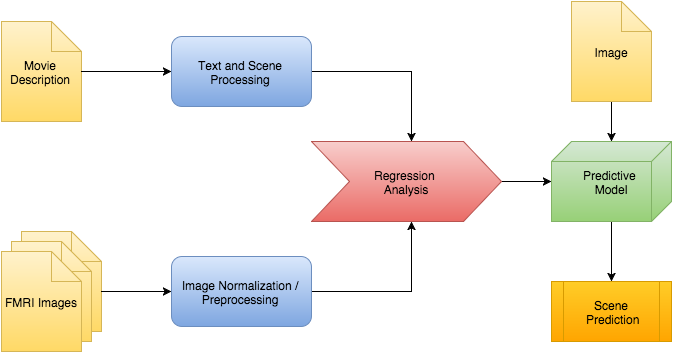
\includegraphics[width=0.6\textwidth]{processflow.png}
\caption{\label{fig:processflow} process flow of the project}
\end{figure}

\subsection{Text Preprocessing}
\par As the movie description as provided was in German, we first used Google
Translate to translate the description to English before proceeding with 
any further processing. Though there may be translational errors, it was decided that it was best to transform the original descriptions (versus using other English descriptions) to maintain the original time stamps from the researchers to have optimal alignment between the description and FMRI data.

\par Due to grammatical differences, we decided to only keep nouns and verbs, and discarded the adjectives and other words including stop-words, which are commonly used words with little meaning or determinable context (e.g. 'and', 'to', 'him'). A publicly available list of stop-words from Princeton University was used for this task. Of the words that remained, a WordNet dictionary was built, which is a popular way to tag words according to a context-specific definition. In this way, words as stand-alone entities will have an unambiguous definition and deeper relationships can be derived from the correlations found. 


 \par After aggregating the set of all contextual definitions of words,
 we build a design matrix composed of the descriptive entries in the movie description. Thus each interval of time with a sentence description of the movie events was treated as a row, and each column represented a context-specific word as a feature. The matrix values are all binary, with a value of '1' indicating that the word is present in the sentence, while '0' indicates that it is not. This was illustrated as a rectangular image with a white square for '1' and black for '0'. As can be seen in Figure 2 below, this matrix is relatively sparse. Finally, in order to format the data such that it correlates explicitly
to the FMRI images, the intervals were split into two-second intervals
to create a one-to-one representation between description objects and images.
\clearpage

\begin{figure}[!htbp]
\centering
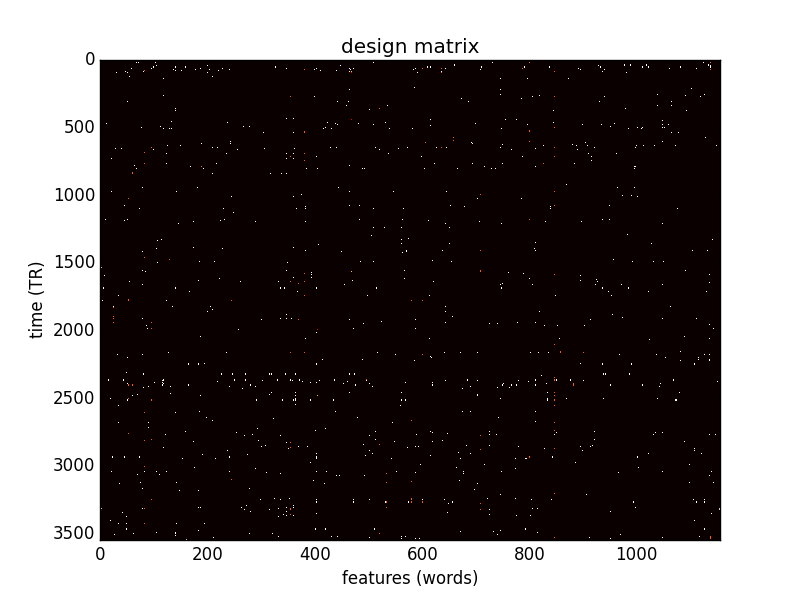
\includegraphics[width=0.5\textwidth]{design_matrix.png}
\caption{\label{fig:design_matrix} A visualization of design matrix for the semantic modeling}
\end{figure}

\subsection{FMRI Preprocessing}
\par We first looked at different measures of spread such as IQR, standard deviation, and RMS for each voxel across time. The following plots below show the standard deviation and RMS differences of the voxel-time courses. It is interesting that the outliers seem to have, to some degree, structure in their location; the outliers seem to clump together in certain places. In order to deal with this, we are going to run different regression models on the BOLD signal and do residual analysis. Hopefully, this will give us a better idea about the correlation structure in our data. We also had to deal with the overlap of movie scenes. More specifically, during the beginning of a new segment/run, researchers replayed the last six seconds of the audiotape of the previous run. To deal with this, we dropped the last four volumes for runs two through seven. We also experimented with PCA. It was hard to extract anything very informative since our dataset is so large. However, when we reach the analysis stage, there is a high chance that PCA will be used (the runtime of some packages may take too long to run on a data set of this size). If this is the case, PCA will potentially allow us to extract the relevant signal areas without sacrificing too much loss of information. 

\begin{figure}
\centering
\begin{minipage}{.5\textwidth}
  \centering
  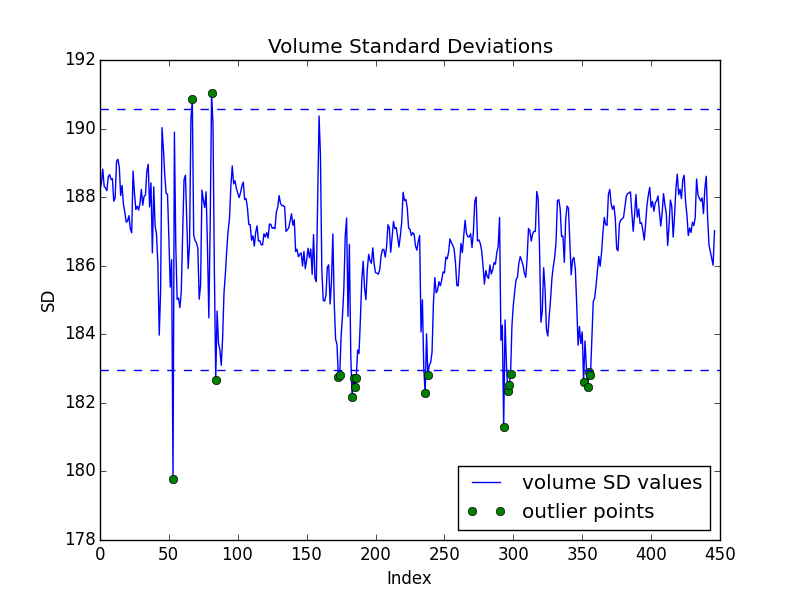
\includegraphics[width=.8\linewidth]{std_plt.png}
  \captionof{figure}{Standard deviation}
  \label{fig:test1}
\end{minipage}%
\begin{minipage}{.5\textwidth}
  \centering
  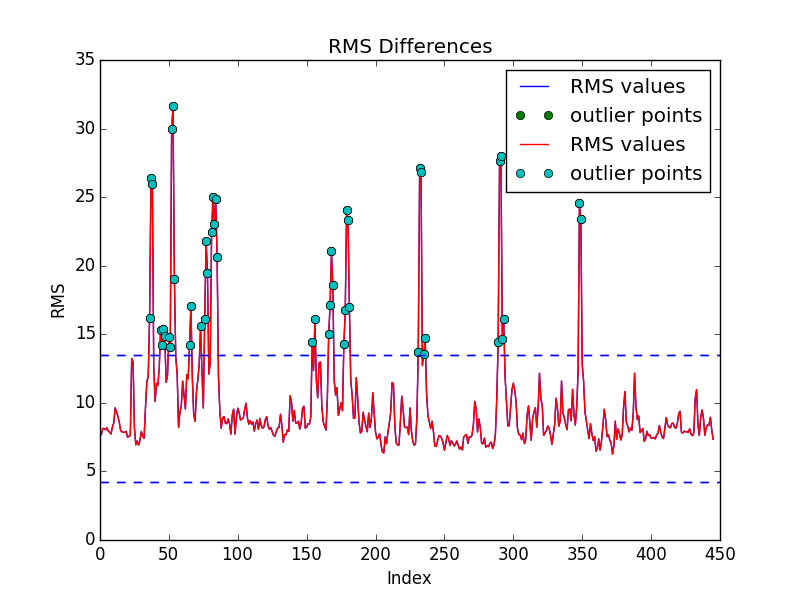
\includegraphics[width=.8\linewidth]{rms_outliers.png}
  \captionof{figure}{RMS(root mean squared differences)}
  \label{fig:test2}
\end{minipage}
\end{figure}
\clearpage

\subsection{Bold response modeling}
\subsubsection{Voxelwise modeling}
\par We use ridge regression for voxelwise modeling of the BOLD response. The entire 8 runs of brain data are separated into training set (7 runs) and validations set (1 run). 7 runs of training set data are further split into 10 groups to do a 10 fold cross-validation on ridge parameters. And finally all the training set of data is used to model with the corresponding part of design matrix to build a voxel-wise ridge regression model. 

\subsubsection{Scene modeling}
\par We were provided a cvs file containing the times at which different scenes occurred in the film. Our goal was to use these scenes as a variant of the the on/off neural task course. Here, we would choose say three scene categories as our stimulus which would comprise the ‘on’ times in the time course for a specific run (all other scenes that occurred during this time interval would be considered ‘off’). With this, we could then check correlations between this time course and the voxel time course, perhaps revealing that certain scenes have different impacts on BOLD signals. We also hope that this will add another layer of comparison between our predictions of words based on BOLD activity.
\begin{figure}[!htbp]
\centering
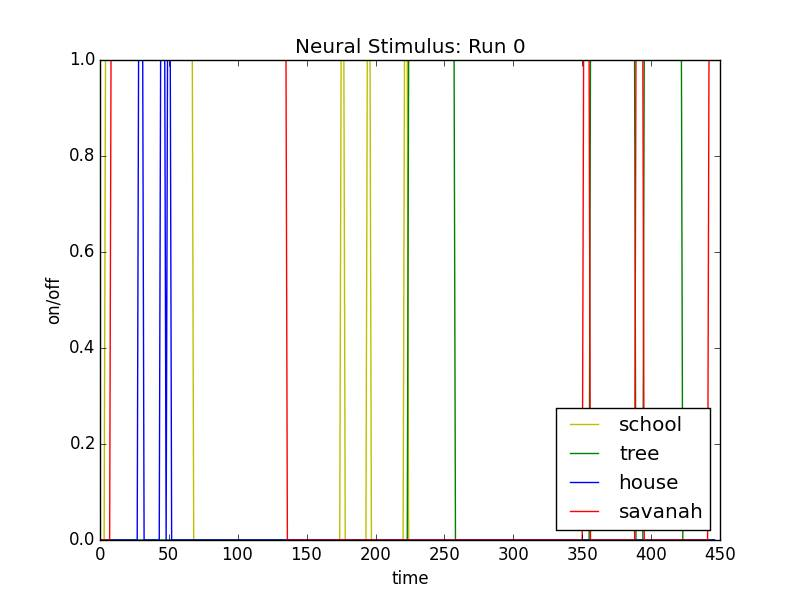
\includegraphics[width=0.7\textwidth]{scenes_conditions.jpg}
\caption{\label{fig:scenes_conditions} An example of scenes conditions across time}
\end{figure}

\subsection{Predictive Testing}
\par In voxel-wise modeling, correlations between predicted BOLD response and actual response are used to evaluate the model performance. Potentially, we could also identify areas that are predicted well by each categories and find the "brain representation" of each semantic categories. Finally, the areas in the brain that are well predicted would be used to predict category labels from BOLD response.

